\chapter{Methods and Implementation}
This chapter focuses on the experimental design and implementation of the artefact,
covering the self-imposed project management methodology, original concept design 
and the overall development process.

\section{Methodology}
When developing software, there are a wide variety of available options to manage the development 
process, which help to structure how time should be allocated as development progresses. 

\subsection{Waterfall} 
\para The first methodology considered was the Waterfall methodology, which is a very common 
approach to software development being sometimes referred to as the Software Development Life Cycle, or SDLC \autocite{adobePopularProjectManagement2023}.
Waterfall is a highly structured and strict methodology which enforces that one stage of development must be completed before the next can begin,
which creates a cascading set of steps, hence its namesake.

\begin{figure}[H]
    \centering
    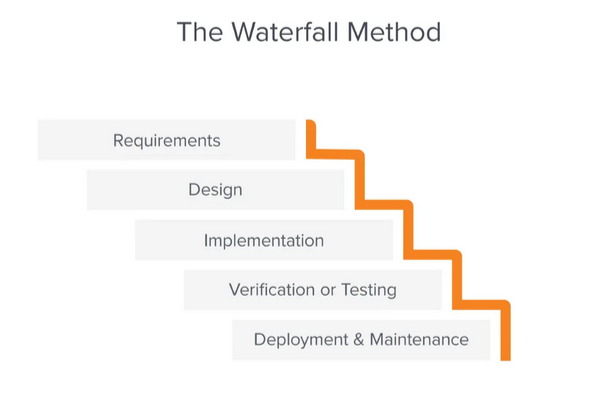
\includegraphics[width=0.8\textwidth]{Implementation/Methodology/Waterfall.png}
    \caption{An overview of a Waterfall workflow \autocite{adobeWaterfallMethodologyProject}. \label{fig:Waterfall}}
\end{figure}

\noindent Waterfall begins by ascertaining all project requirements for all stages of the project, which 
would include costs, risks, associated dependencies and overall timelines for completions of each stage.
Following this is the design stage, where a general high-level design is created to demonstrate the 
project, and this design is then acted upon and implemented in the implementation stage. Then, the 
implementation is rigorously tested before its eventual deployment.

\para It is a methodology with a strong reputation due to its clear structure, with all necessary facts and figures 
being calculated in the requirements stage before any designs or development occur. The clear structure allows 
progress to be easily measured against each predefined milestone.

\para Though, despite these advantages, Waterfall brings with it some clear disadvantages - the first of which 
being that with all requirements being defined at the very beginning of the project's development,
it introduces significant difficulty should there be any further requirements specified during development. This would also 
bring in the second disadvantage known as 'deadline creep' \autocite{adobeWaterfallMethodologyProject}; 
if one stage is delayed, such as by request for additional features, this would then impact all subsequent stages. 

\subsection{Agile}
The second methodology considered was another highly reputed software development methodology known as Agile.
Unlike Waterfall which defines all stages and requirements at the beginning, Agile is a highly iterative methodology with steps
known as 'sprints' which are frequently repeated, providing a more incremental approach to development. Each of these sprints
would represent a small part of the program, eventually building up to the full version.

\para As depicted in Figure \ref{fig:ExampleAgileSprint}, 
Agile sprints begin by planning the overall aims of that particular sprint. Similarly to Waterfall, a high-level
design is then created and developed, before being rigorously tested. This is also one of Agile's key benefits; the 
constant testing of the small parts developed in each sprint helps ensure that all bugs can be rectified, unlike 
Waterfall where the whole product is tested and some smaller elements with bugs could potentially be overlooked.
After testing, the product of that sprint is deployed and reviewed. Then, the cycle begins anew with another 
sprint.

\begin{figure}[H]
    \centering
    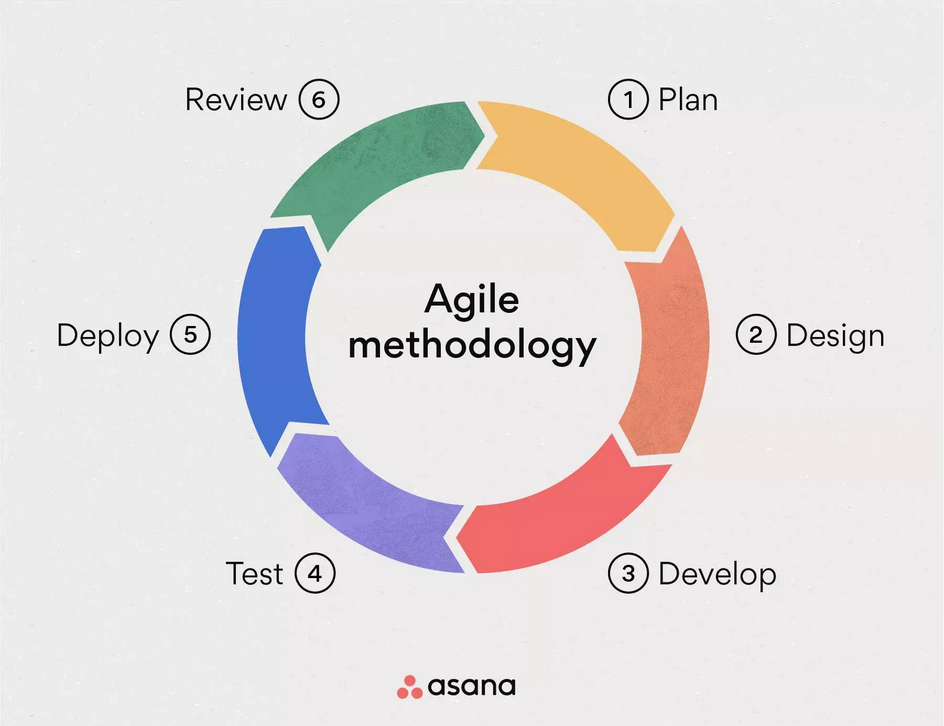
\includegraphics[width=0.65\textwidth]{Implementation/Methodology/Agile.png}
    \caption{An overview of an Agile sprint \autocite{asanaWhatAgileMethodology}\label{fig:ExampleAgileSprint}}
\end{figure}


\noindent The most prominent key benefit of Agile is its sprint-based iterative nature that allows for requirements to shift 
throughout development without major disruption. Furthermore, this incremental process minimises the risk of total project 
failure as usable components are constantly produced. In business environments, Agile also allows for enhanced teamwork, though 
this will not be present in this particular project.

\para As with Waterfall, Agile is not without drawbacks. Agile's most notable drawback is known as 'scope creep' \autocite{malsamWhatScopeCreep2024},
which occurs when requirements are continually added to a point where development can never truly end; the product continues to expand 
far beyond its original intentions to the point where maintenance becomes extremely difficult or outright impossible with an 
ever-expanding codebase. Furthermore, it is possible that because of this, the end product can be almost entirely different to its original concept.

\subsection{Comparison and decision}

Both methodologies bear strong benefits and drawbacks. The particular choice for this project is Agile, primarily because of the reduced 
risk through constant testing and also for its deeply flexible nature allowing the requirements of the project to potentially shift 
over time as needed, unlike Waterfall where this could cause major deadline creep. Additionally, the time-sensitive nature of this project 
best suits Agile's fast incremental sprints rather than the slower, more methodical Waterfall.

\section{Potential limitations}
The project as a whole bears some limitations of its own that may hinder the development process or the final product.

\subsection{Time}
The project is likely to take a considerable amount of time to develop to the excellent standard desired. This poses an issue 
in balancing time throughout the academic year alongside four other modules each with their own independent deadlines and workloads
of similar scale. As such, it is possible that if the product has issues, they could have been remedied with additional development 
time.

\subsection{Cost}
Due to the inability to use OpenAI's LLMs on a local device because of both their proprietary nature and extreme hardware requirements,
their public API will need to be used instead. This incurs a financial cost for every query sent and response received from the LLM,
dependent on the model chosen. For example, GPT-4o has a cost of \$2.50 per 1,000,000 tokens. Throughout the development and testing 
processes in each sprint, a cost will slowly begin to accrue.

\subsection{Experience}
Personally, I have never worked with LLM APIs before, nor the frameworks used to create apps with them such as LangChain. As such,
it is highly likely that many issues will be faced during the development process as I am forced to learn a tech stack that is completely 
new to me. This also links back to the previously mentioned time constraint, with the time taken to learn the modules used being time that 
could have been spent on development had I known them ahead of time.

\subsection{Independence}
This project is a solo venture with no support from others. As such, the previously mentioned issues of time and cost are entirely 
my own burden and responsibility. 

\subsection{LLM Unpredictability}
LLMs are an extremely useful tool, being able to execute instructions given to them in natural language. However, without specific tuning, 
an LLM will not give the same response to the same prompt every time it is given. While this does add a sense of personality which could 
aid with a chatbot, it may risk answering questions incorrectly. This also can make LLM-based programs extremely challenging to debug due 
to this lack of reproducibility.

\subsection{LangChain Documentation}
LangChain will be a critical element in this project's development, serving as the backend framework that the chatbot will run on.
Therefore, it is mandatory that I learn about it in order to produce a functional product, which would typically involve reading the 
documentation as is common when learning new modules. However, LangChain's documentation is frequently outdated and/or references 
functions or classes that have since been deprecated, without the documentation being updated. LangChain also frequently deprecates classes 
and functions with each new update, meaning that finding what currently works is a challenge in itself.


\section{Design}
Before any design concepts can be created, it is first necessary to establish what is being designed. Therefore, the functional and 
non-functional requirements for the chatbot were considered.

\subsection{Requirements}\label{sec:Requirements}
\subsubsection{Functional Requirements}
The following requirements are deemed essential to the chatbot's function, and the project cannot be considered complete unless they 
are fulfilled:

\begin{itemize}
    \item The chatbot must interpret and respond to answers in English.
    \item The chatbot must accept text queries.
    \item The chatbot must respond using text.
    \item The chatbot must be accessible at all times.
    \item The chatbot must supply BCU-related information.
    \item The chatbot must answer at least 75\% of BCU-related queries correctly.
    \item The chatbot must have a GUI for ease of use and accessibility.
    \item Multiple users must be able to use the chatbot at the same time.
\end{itemize}

\subsubsection{Non-functional Requirements}
The following requirements, while not essential, would be beneficial if fulfilled:

\begin{itemize}
    \item The chatbot should respond to queries within 10 seconds.
    \item The chatbot could allow for voice input and output.
    \item The chatbot could be deployed on an existing messaging service such as Teams.
\end{itemize}

% \subsection{Conceptual solution}
% The proposed solution and final artefact for this project will be an LLM-based chatbot with RAG capabilities to query 
% a vector store of embedded university-related data. Users will be able to access the chatbot and send questions to it 
% pertaining to Birmingham City University, such as information about its campus locations and various policies that impact 
% them as students. The chatbot will interpret their natural language queries and retrieve relevant information from official
% University sources.

% Based on this understanding of what the proposed solution is, a sequence of events necessary for the project's completion 
% can be created:

% \begin{itemize}
%     \item 
% \end{itemize}


\subsection{Conceptual flowchart}
The flowchart presented in Figure XXX depicts a model interaction from the user's perspective.
%\ref{fig:ConceptFlowchartUser}

\begin{tcolorbox}[colback=red!5!white,colframe=red!75!black,title=Not present in draft]
    Time constraints on this draft meant I simply don't have time to make this diagram.
\end{tcolorbox}

\noindent In the interest of saving costs and reducing response times, the chatbot will ideally not query its university information vector store 
unless it cannot answer a question without it. This is because appending the university information, even in small amounts, would 
greatly increase the token usage of each individual prompt. This decision functionality would be provided by LangGraph, and is detailed 
further in Section \ref{sec:ChatbotBackend}.

\subsection{Wireframes}
The wireframe presented in Figure XXX depicts an early concept of how the chatbot's GUI could look like.
%\ref{fig:OriginalWireframe}

\begin{tcolorbox}[colback=red!5!white,colframe=red!75!black,title=Not present in draft]
    Time constraints on this draft meant I simply don't have time to make this diagram.
\end{tcolorbox}

\noindent Users will have a clearly labelled text input box, and a messaging interface similar to other text messaging apps 
which they would hopefully be familiar with allowing for them to quickly understand how to interact with the chatbot.